% Fixing: Too many math alphabets used in version normal.
\newcommand\hmmax{0}
\newcommand\bmmax{0}
\documentclass[12pt]{article}
\usepackage[left=1.0cm,top=1.5cm,right=1.0cm,bottom=1.5cm]{geometry}
\usepackage{parskip}
\usepackage{framed}
\usepackage{enumitem}
\usepackage[numbers]{natbib}
\usepackage{trimclip}
\makeatletter
\DeclareRobustCommand{\circbullet}{\mathbin{\vphantom{\circ}\text{\circbullet@}}}
\newcommand{\circbullet@}{%
  \check@mathfonts
  \m@th\ooalign{%
    \clipbox{0 0 0 {\dimexpr\height-\fontdimen22\textfont2}}{$\bullet$}\cr
    $\circ$\cr
  }%
}
\DeclareRobustCommand{\bulletcirc}{\mathbin{\text{\bulletcirc@}}}
\newcommand{\bulletcirc@}{%
  \check@mathfonts
  \m@th\ooalign{%
    \raisebox{\fontdimen22\textfont2}{\clipbox{0 {\fontdimen22\textfont2} 0 0}{$\bullet$}}\cr
    $\circ$\cr
  }%
}
\makeatother

% https://tex.stackexchange.com/questions/648845/sans-serif-uppercase-greek-no-longer-showing-in-acmart
\DeclareMathAlphabet{\mathsf}{OT1}{LibertinusSans-LF}{m}{n}
\SetMathAlphabet{\mathsf}{bold}{OT1}{LibertinusSans-LF}{bx}{n}
\DeclareMathAlphabet{\mathtt}{OT1}{lmtt}{m}{n}
\SetMathAlphabet{\mathtt}{bold}{OT1}{lmtt}{bx}{n}


\usetikzlibrary{calc,decorations.pathmorphing,shapes,positioning}
\newcounter{sarrow}
\newcommand\xrsquigarrow[1]{%
\stepcounter{sarrow}%
\mathrel{\begin{tikzpicture}[baseline= {( $ (current bounding box.south) + (0,-0.5ex) $ )}]
\node[inner sep=.5ex] (\thesarrow) {$\scriptstyle #1$};
\path[draw,<-,decorate,
  decoration={zigzag,amplitude=0.7pt,segment length=1.2mm,pre=lineto,pre length=4pt}]
    (\thesarrow.south east) -- (\thesarrow.south west);
\end{tikzpicture}}%
}
\makeatletter
\newcommand{\xRightarrow}[2][]{\ext@arrow 0359\Rightarrowfill@{#1}{#2}}
\makeatother

\newcommand{\thmref}[1]{\cref{#1}~(\nameref{#1})}
\newcommand{\Thmref}[1]{\Cref{#1}~(\nameref{#1})}

%%%%
% TODO macros
\newcommand{\MK}[1]{\todo[color=orange!30]{TODO: #1}}
\newcommand{\MKin}[1]{\todo[color=orange!30,inline]{TODO: #1}}
\newcommand{\MP}[1]{\todo[color=blue!30]{TODO: #1}}
\newcommand{\MPin}[1]{\todo[color=blue!30,inline]{TODO: #1}}
\newcommand{\hltt}[1]{\begin{center}\fbox{\color{green}\large{#1}}\end{center}}

% Approx
\newcommand{\pages}[1]{}%\xspace\todo{\textbf{($\sim$#1 pages)}\xspace}}

%%%%
% Colors
\newcommand{\neutcol}[0]{black}
\newcommand{\stlccol}[0]{RoyalBlue}
\newcommand{\irccol}[0]{Apricot}
\newcommand{\ulccol}[0]{RedOrange}
\newcommand{\objcol}[0]{Emerald} %CarnationPink}
\newcommand{\commoncol}[0]{black}

\newcommand{\col}[2]{\ensuremath{{\color{#1}{#2}}}}

\newcommand{\com}[1]{\ensuremath\mathit{\col{\neutcol}{#1}}}
\newcommand{\src}[1]{\ensuremath\mathsf{\col{\stlccol}{#1}}}
\newcommand{\irl}[1]{\ensuremath\mathit{\col{\irccol}{#1}}}
\newcommand{\trg}[1]{\ensuremath\mathbf{\col{\ulccol}{#1}}}
\newcommand{\obj}[1]{\ensuremath\mathtt{\col{\objcol}{#1}}}

%%%%
% Text Decorations
\newcommand\BrText[2]{%
  \par\smallskip
   \noindent\makebox[\textwidth][r]{$\text{\scriptsize #1}\left\{
    \begin{minipage}{\textwidth}
    #2
    \end{minipage}
  \right.\nulldelimiterspace=0pt$}\par\smallskip
}
\newcommand{\mi}[1]{\ensuremath{\mathit{#1}}}
\newcommand{\mr}[1]{\ensuremath{\mathrm{#1}}}
\newcommand{\mt}[1]{\ensuremath{\texttt{#1}}}
\newcommand{\mtt}[1]{\ensuremath{\mathtt{#1}}}
\newcommand{\mf}[1]{\ensuremath{\mathbf{#1}}}
\newcommand{\mk}[1]{\ensuremath{\mathfrak{#1}}}
\newcommand{\mc}[1]{\ensuremath{\mathcal{#1}}}
\newcommand{\ms}[1]{\ensuremath{\mathsf{#1}}}
\newcommand{\mb}[1]{\ensuremath{\mathbb{#1}}}
\newcommand{\msc}[1]{\ensuremath{\mathscr{#1}}}

\newcommand{\bul}[1]{{\setulcolor{RoyalBlue}\ul{#1}}}
\newcommand{\rul}[1]{{\setulcolor{RedOrange}\ul{#1}}}
\newcommand{\iul}[1]{{\setulcolor{Apricot}\ul{#1}}}
\newcommand{\oul}[1]{{\setulcolor{Emerald}\ul{#1}}}
\newcommand{\pul}[1]{{\setulcolor{CarnationPink}\ul{#1}}}

\newcommand{\lock}{\ensuremath\text{\scriptsize\faIcon{lock}}}
\newcommand{\unlock}{\ensuremath\text{\scriptsize\faIcon{lock-open}}}

\newcommand{\tup}[2]{\ensuremath (#1 %
  \readlist\myterms{#2}%
  \foreachitem\x\in\myterms{;\x}%
  )%
}

\newcommand{\isdef}[0]{\ensuremath{\mathrel{\overset{\makebox[0pt]{\mbox{\normalfont\tiny\sffamily def}}}{=}}}}

%%%%
% List of contributions
\newcounter{contrib}
\newcommand{\contribnum}[0]{\stepcounter{contrib}{\arabic{contrib}}.~}
\newcommand{\contribution}[1]{\smallskip\noindent\textbf{{#1.}\xspace}}

%%%%
% A symbol for Coq-verified theorems.
\newcommand{\BareCoqSymbol}{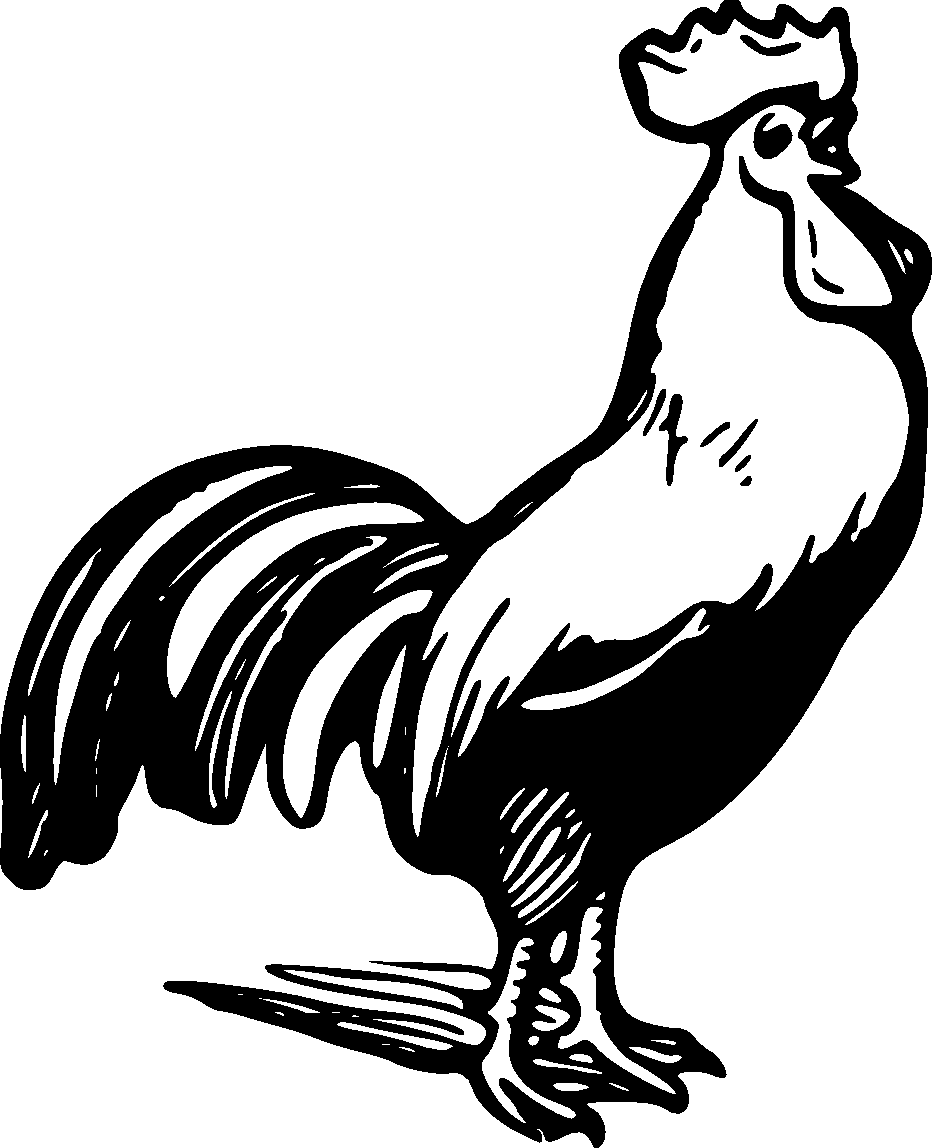
\includegraphics[height=0.9em]{coq.pdf}}
\newcommand{\CoqSymbol}{\raisebox{-.2ex}{\BareCoqSymbol\,}}
\newcommand{\Coqed}{\hfill\CoqSymbol}

\newcommand{\BareInvCoqSymbol}{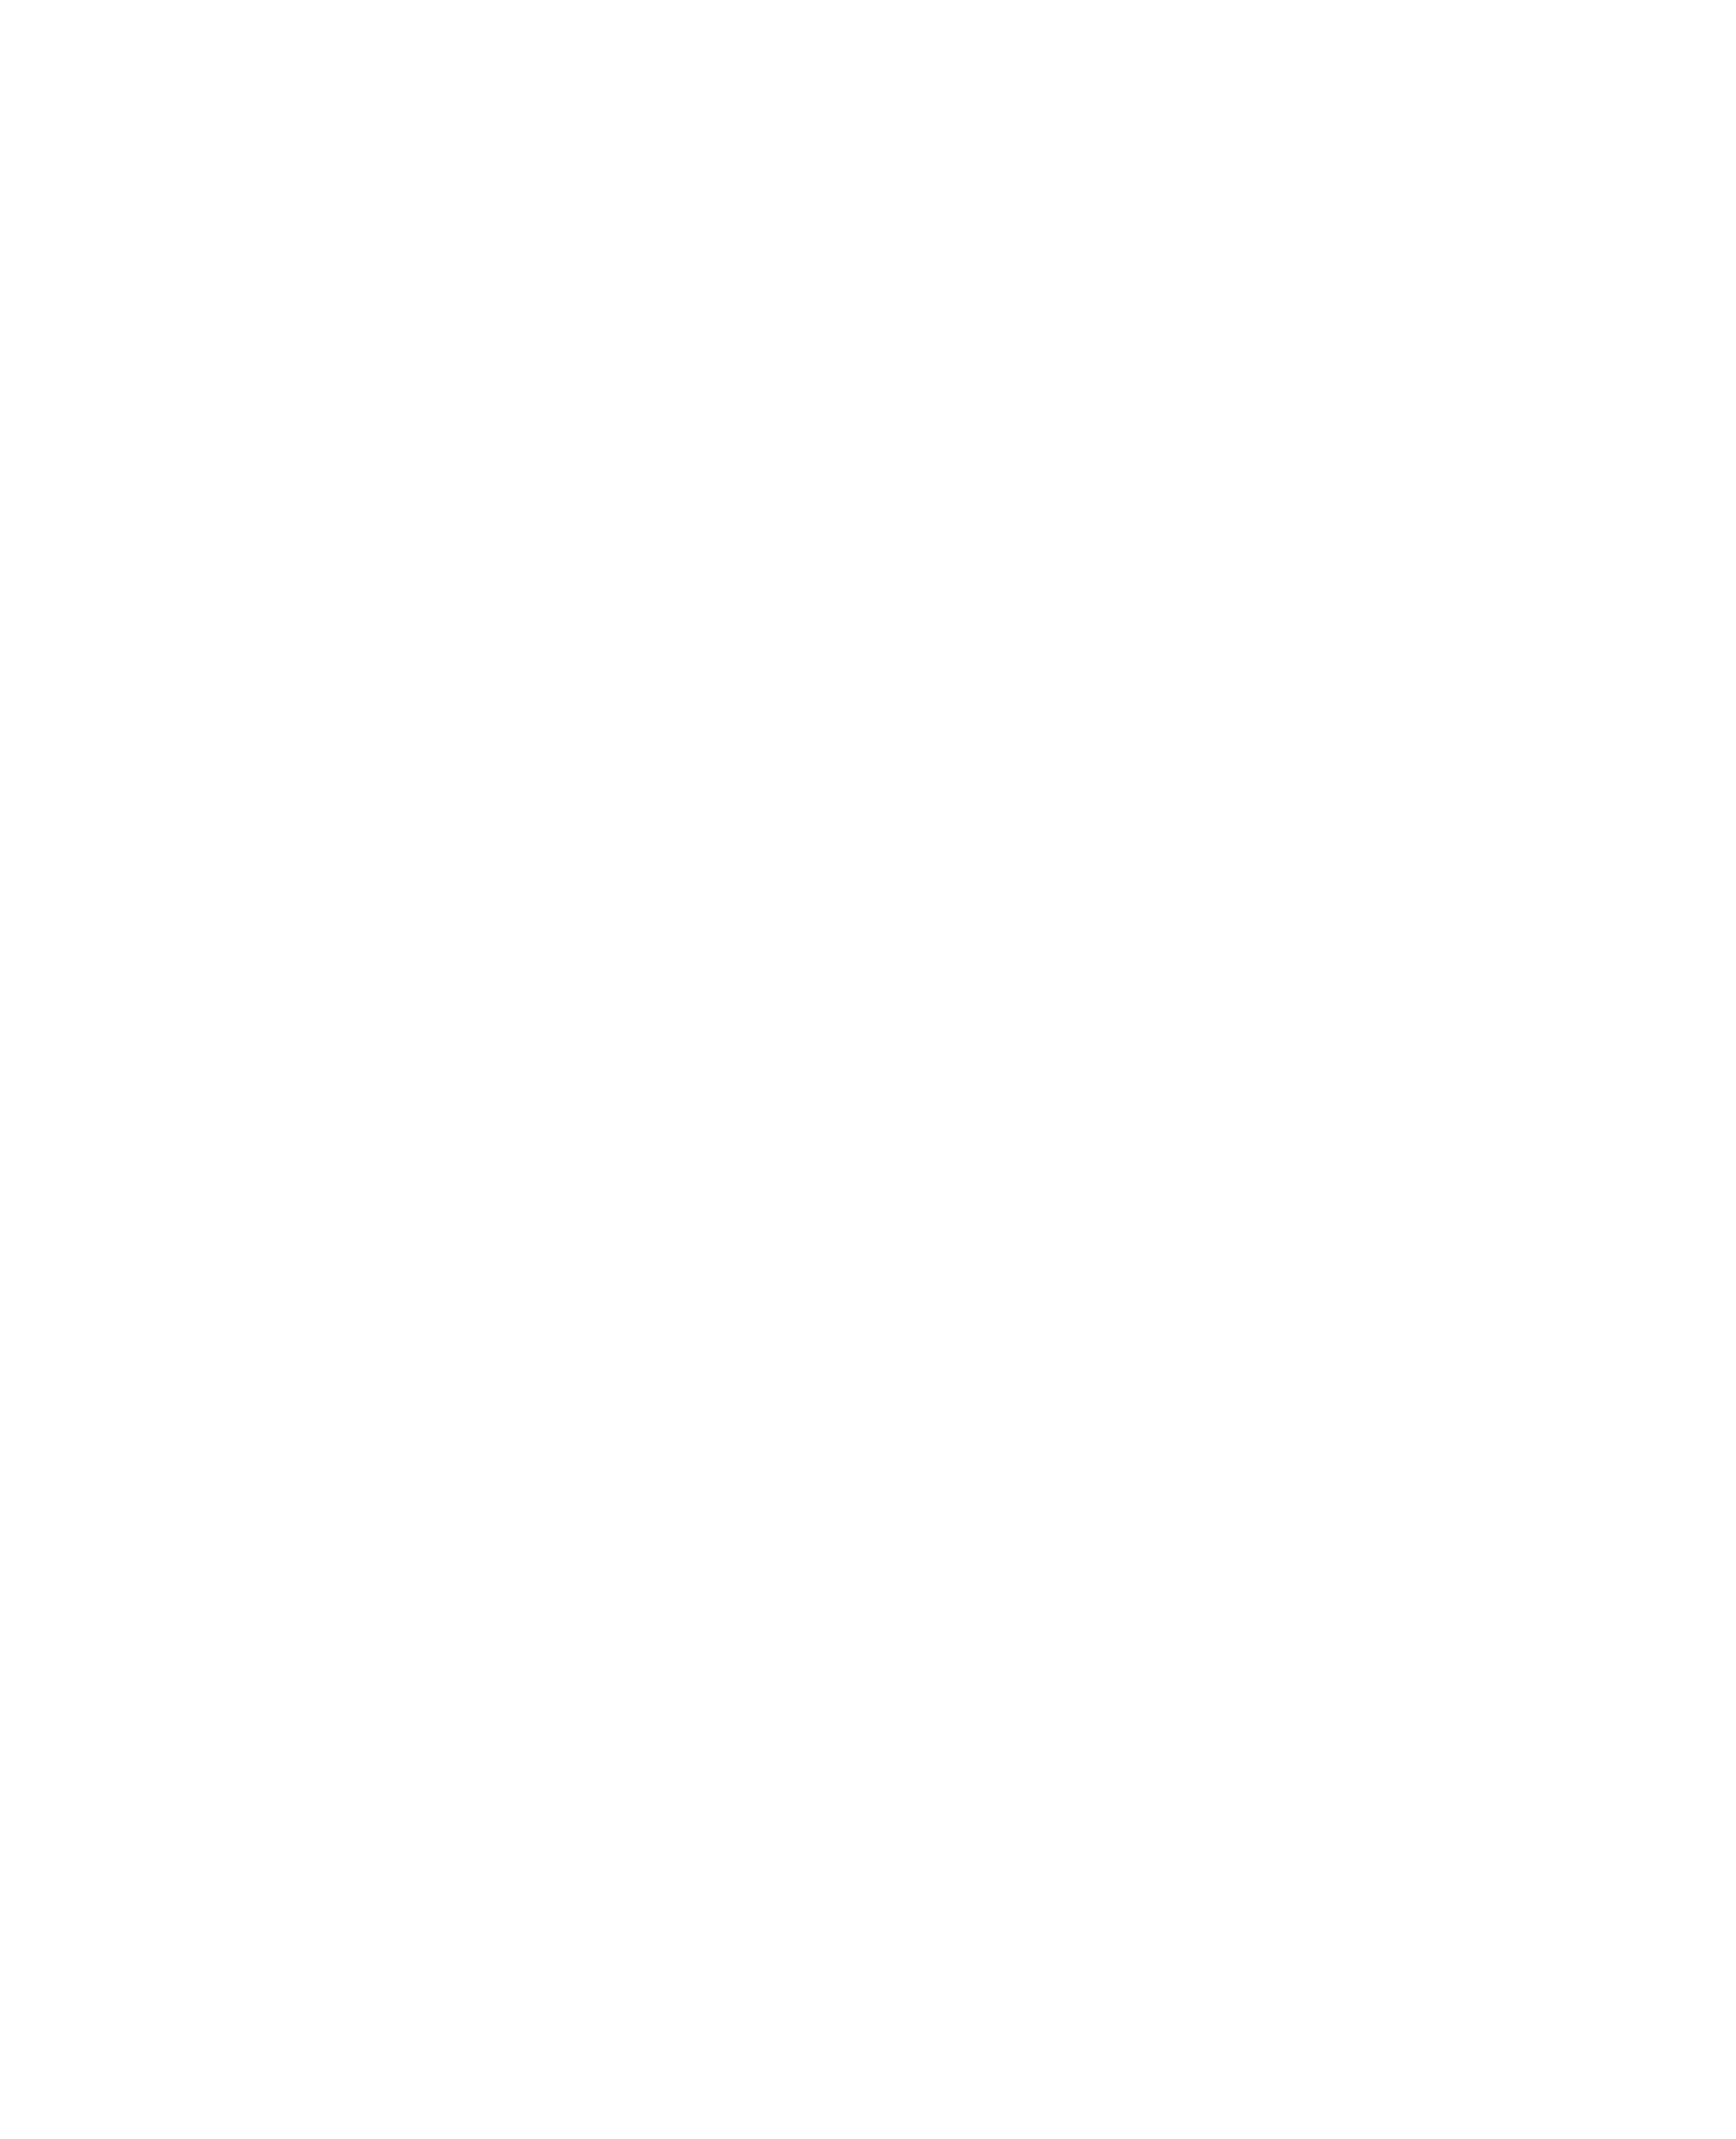
\includegraphics[height=0.9em]{inv_coq.png}}
\newcommand{\InvCoqSymbol}{\raisebox{-.2ex}{\BareInvCoqSymbol\,}}

%%%%
% Typerules
\newcommand{\textgraybox}[1]{\boxed{#1}}
\newdimen\zzfontsz
\newcommand{\fontsz}[2]{\zzfontsz=#1%
{\fontsize{\zzfontsz}{1.2\zzfontsz}\selectfont{#2}}}
\newcommand{\mathsz}[2]{\text{\fontsz{#1}{$#2$}}}
\newcommand{\instsymColon}{%
     \raisebox{-0.09ex}{\text{\normalfont{:}}}}
\newcommand{\judgboxfontsize}[1]{%
        \mathsz{11pt}{#1}%
}
\newcommand{\judgbox}[2]{%
      {\raggedright \textgraybox{\ensuremath{\judgboxfontsize{#1}}}\!%
        \fontsz{9pt}{\begin{tabular}[c]{l} #2 \end{tabular}} %
}}
\newcounter{typerule}
\crefname{typerule}{rule}{rules}

\newcommand{\typeruleInt}[5]{%
	\def\thetyperule{#1}%
	\refstepcounter{typerule}%
	\label{tr:#4}%
	%
  \ensuremath{\begin{array}{c}#5 \inference{#2}{#3}\end{array}}
}
\newcommand{\typerule}[4]{%
  \typeruleInt{#1}{#2}{#3}{#4}{\textsf{\scriptsize ({#1})} \\      }
}
\newcommand{\typerulenolabel}[3]{%
	\def\thetyperule{#1}%
	\refstepcounter{typerule}%
  \ensuremath{\begin{array}{c} \inference{#2}{#3}\end{array}}
}
\newcommand{\typerulederiv}[3]{%
  \ensuremath{\begin{array}{c} \inference{#2}{#3} #1\end{array}}
}

%%%%
% Language-specific definitions
% names of properties
\newcommand{\tmssafe}{\ensuremath\operatorname{tms}}
\newcommand{\smssafe}{\ensuremath\operatorname{sms}}
\newcommand{\mssafe}{\ensuremath\operatorname{ms}}
\newcommand{\scctsafe}{\ensuremath\operatorname{scct}}
\newcommand{\msscctsafe}{\ensuremath\operatorname{msscct}}

% Languages
\newcommand{\Ltms}{\ensuremath\src{L_{\tmssafe}}}
\newcommand{\Ltrg}{\ensuremath\trg{L}}
\newcommand{\Lms}{\ensuremath\irl{L_{\mssafe}}}
\newcommand{\Lscct}{\ensuremath\obj{L_{\scctsafe}}}

% Traces
\newcommand{\event}[1][]{a#1}
\newcommand{\absevent}[1][]{\ensuremath\bm{\event[#1]}}
\newcommand{\emptyevent}{\ensuremath\varepsilon}
\newcommand{\trace}[1][]{\ensuremath\overline{a#1}}
\newcommand{\class}[1][]{\ensuremath\mb{C}}
\newcommand{\lift}[1]{\ensuremath\lfloor\xspace{#1}\xspace\rfloor}
\newcommand{\hole}[1]{\ensuremath{\left[#1\right]}}
\newcommand{\ev}[1]{\text{#1}}
\newcommand{\absev}[1]{\ensuremath\bm{#1}}
\newcommand{\abstrace}[1][]{\ensuremath\bm{\trace[]}#1}
\newcommand{\absterm}{\ensuremath\lightning{\kern-5.5pt}\lightning}

% Trace Relations
\newcommand{\traceagree}[4][^*]{\ensuremath{#3}\cong_{#2}#1{#4}}
\newcommand{\tmstraceagree}[3][^*]{\traceagree[#1]{\tmssafe}{#2}{#3}}
\newcommand{\smstraceagree}[3][^*]{\traceagree[#1]{\smssafe}{#2}{#3}}
\newcommand{\mstraceagree}[3][^*]{\traceagree[#1]{\mssafe}{#2}{#3}}
\newcommand{\sccttraceagree}[3][^*]{\traceagree[#1]{\scctsafe}{#2}{#3}}

% Monitors
\newcommand{\monitor}[1][]{\ensuremath T#1}
\newcommand{\tmsmonitor}[1][]{\monitor[_{TMS}{#1}]}
\newcommand{\smsmonitor}[1][]{\monitor[_{SMS}{#1}]}
\newcommand{\scctmonitor}[1][]{\monitor[_{sCCT}{#1}]}
\newcommand{\msmonitor}[1][]{\monitor[_{MS}{#1}]}
\newcommand{\monitorcheck}[4][{\kern-3.5pt}^*]{%
  \vdash\xspace{#2}\xspace \xrsquigarrow{#4}{#1}\xspace{#3}\xspace%
}
\newcommand{\monsafe}[2]{\ensuremath\vdash_{mon}{#1}:{#2}}

\newcommand{\abssecuritytag}[1][]{\ensuremath\bm{\sigma}#1}

\newcommand{\montmssafe}[1]{\monsafe{#1}{\tmssafe}}
\newcommand{\monsmssafe}[1]{\monsafe{#1}{\smssafe}}
\newcommand{\monmssafe}[1]{\monsafe{#1}{\mssafe}}
\newcommand{\monscctsafe}[1]{\monsafe{#1}{\scctsafe}}
\newcommand{\monmsscctsafe}[1]{\monsafe{#1}{\msscctsafe}}

% Languages
\newcommand{\LTMS}{\src{L_{TMS}}}
\newcommand{\LT}{\trg{L}}
\newcommand{\LMS}{\irl{L_{MS}}}
\newcommand{\LCCT}{\obj{L_{sCCT}}}

\newcommand{\bnfdef}{\ensuremath{\mathrel{::=}}}

% Substitution
\newcommand{\subst}[2]{\ensuremath \hole{#1\text{ for }#2}}
\newcommand{\substvar}[1][]{\ensuremath \gamma#1}
\newcommand{\substlist}[1][]{\ensuremath \overline{\gamma#1}}

\newcommand{\partialeval}[2]{\ensuremath \operatorname{\mathtt{mix}}(#1, #2)}

% Predefined Sets
\newcommand{\nat}{\ensuremath\mb{N}}

% Types
\newcommand{\natt}{\ensuremath\mb{N}_t\xspace}
\newcommand{\ptrqual}[1][]{\ensuremath\xspace q#1\xspace}
\newcommand{\fullq}{1\xspace}
\newcommand{\halfq}{\sfrac{1}{2}\xspace}
\newcommand{\ptrn}[1][\ptrqual]{\ensuremath\xspace ref_{#1}\ \natt\xspace}
\newcommand{\wptr}{\ensuremath\ptrn[\halfq]\xspace}
\newcommand{\ptr}{\ensuremath\ptrn[\fullq]\xspace}
\newcommand{\type}[1][]{\ensuremath\tau#1\xspace}
\newcommand{\typenv}[1][]{\ensuremath\Gamma#1\xspace}

% Terms
\newcommand{\wrapkeyword}[2][]{\ensuremath{#1{#2}}}
\newcommand{\expr}[1][]{e#1\xspace}
\newcommand{\ectx}[1][]{K#1\xspace}
\newcommand{\finalexpr}[1][]{f#1\xspace}
\newcommand{\valueexpr}[1][]{v#1\xspace}
\newcommand{\lbinop}[3][]{\ensuremath {#2}{#1{\oplus}}{#3}\xspace}
\newcommand{\lget}[3][]{\ensuremath #2{#1{[}}{#3}{#1{]}}\xspace}
\newcommand{\lset}[4][]{\ensuremath #2{#1{[}}{#3}{#1{]\leftarrow}}#4\xspace}
\newcommand{\lnew}[3][]{\ensuremath \wrapkeyword[#1]{new}\ #2\ {#1{[}}#3{#1{]}}\xspace}
\newcommand{\llet}[4][]{\ensuremath \wrapkeyword[#1]{let}\ #2 {#1{=}} #3\ \wrapkeyword[#1]{in}\ #4\xspace}
\newcommand{\ldelete}[2][]{\ensuremath \wrapkeyword[#1]{delete}\ #2\xspace}
\newcommand{\lreturn}[2][]{\ensuremath \wrapkeyword[#1]{return}\ #2\xspace}
\newcommand{\lcall}[3][]{\ensuremath \wrapkeyword[#1]{call}\ #2\ #3\xspace}
\newcommand{\lifz}[4][]{\ensuremath \wrapkeyword[#1]{ifz}\ #2\ \wrapkeyword[#1]{then}\ #3\ \wrapkeyword[#1]{else}\ #4\xspace}
\newcommand{\labort}[1][]{\ensuremath \wrapkeyword[#1]{abort()}\xspace}
\newcommand{\lispoisoned}[2][]{\ensuremath #2\ \wrapkeyword[#1]{is\ }{#1{\poisoned}}\xspace}
\newcommand{\lpair}[3][]{\ensuremath {#1{\langle}} #2 {#1{;}} #3 {#1{\rangle}} \xspace}
\newcommand{\lproja}[2][]{\ensuremath {#2}{#1{.0}} \xspace}
\newcommand{\lprojb}[2][]{\ensuremath {#2}{#1{.1}} \xspace}
\newcommand{\lhast}[3][]{\ensuremath {#2}\ \wrapkeyword[#1]{has}\ #3 \xspace}
\newcommand{\lwrdoit}[2][]{\ensuremath \wrapkeyword[#1]{wrdoit}\ #2\xspace}
\newcommand{\lrddoit}[3][]{\ensuremath \wrapkeyword[#1]{rddoit}\ #2\ \wrapkeyword[#1]{in}\ #3\xspace}
\newcommand{\function}[1][]{F#1\xspace}
\newcommand{\lfunction}[4][]{\ensuremath\wrapkeyword[#1]{fn}\ {#2}\ {#3}\ {#1{:=}}\ #4\xspace}
\newcommand{\prog}[3][]{\ensuremath\wrapkeyword[#1]{\langle}\ #2; #3\wrapkeyword[#1]{\rangle}\xspace}

% Compiler
\newcommand{\rtp}[2]{\ensuremath\vdash{#1}:{#2}}
\newcommand{\ccbase}[1][]{\ensuremath\gamma{#1}}
\newcommand{\cc}[3][]{\ensuremath{\ccbase[#1]}^{#2}_{#3}\xspace}
\newcommand{\cca}{\ensuremath\cc{\Ltms}{\Ltrg}}
\newcommand{\ccb}{\ensuremath\cc{\Ltrg}{\Lms}}
\newcommand{\ccdce}{\ensuremath\cc[_{\gls{dce}}]{\Lms}{\Lms}}
\newcommand{\cccf}{\ensuremath\cc[_{\gls{cf}}]{\Lms}{\Lms}}
\newcommand{\ccscct}{\ensuremath\cc{\Lms}{\Lscct}}
\newcommand{\ccmsscct}{\ensuremath\cc{\Ltms}{\Lscct}}

% Backtranslation
\newcommand{\backbase}[1][]{\ensuremath\wp#1}
\newcommand{\backt}[3][]{\ensuremath{}^{#2}_{#3}\backbase[#1]}

% Satisfaction
\newcommand{\contextvar}[1][]{C#1}
\newcommand{\progvar}[1][]{p#1}
\newcommand{\wholeprogvar}[1][]{w#1}
\renewcommand{\class}[1][]{\mathbb{C}#1}
\newcommand{\link}[2]{\ensuremath\operatorname{link}\left({#1};{#2}\right)}
\newcommand{\behav}[1]{\ensuremath\operatorname{behav}\left({#1}\right)}
\newcommand{\sat}[2]{\ensuremath\vdash{#1}:{#2}}
\newcommand{\rsat}[2]{\ensuremath\vdash_R{#1}:{#2}}

% State
\newcommand{\securitytag}[1][]{\ensuremath\sigma#1}
\newcommand{\sandboxtag}[1][]{t#1}
\newcommand{\ctx}{\text{ctx}}
\newcommand{\comp}{\text{comp}}
\newcommand{\loc}[1][]{\ensuremath l#1}
\newcommand{\poison}{\ensuremath\rho}
\newcommand{\poisoned}{\ensuremath\text{\Biohazard}}
\newcommand{\poisonless}{\ensuremath\square}
\newcommand{\store}[1][]{\ensuremath\Delta#1}
\newcommand{\storeel}[5]{\ensuremath #1\mapsto\tup{#2}{#3,#4,#5}}
\newcommand{\comm}[1][]{\ensuremath c#1}
\newcommand{\ctxtocomp}{\ensuremath\xspace ? \xspace}
\newcommand{\comptoctx}{\ensuremath\xspace ! \xspace}
\newcommand{\nocomm}{\ensuremath\xspace \varnothing \xspace}
\newcommand{\heap}[1][]{\ensuremath H#1}
\newcommand{\ectxstack}[1][]{\ensuremath\overline{\ectx#1}}
\newcommand{\library}[1][]{\ensuremath\Xi#1}
\newcommand{\commlib}[1][]{\ensuremath\xi#1}
\newcommand{\cfstate}[1][]{\ensuremath\Psi#1}
\newcommand{\memstate}[1][]{\ensuremath\Phi#1}
\newcommand{\statevar}[1][]{\ensuremath\Omega#1}
\newcommand{\rtt}[2]{\ensuremath #1 \triangleright #2}
\newcommand{\growh}[2]{\ensuremath #1 \ll #2}
\newcommand{\seth}[3]{\ensuremath #1(#2 \mapsto #3)}

% Various Judgements
\newcommand{\fresh}[2]{\ensuremath{#1}\vdash{#2}\xspace\operatorname{fresh}\xspace}
\newcommand{\tcheck}[3]{\ensuremath{#1}\vdash{#2}:{#3}\xspace}
\newcommand{\notowned}[1]{\ensuremath\vdash{#1}\xspace\operatorname{not-owned}\xspace}
\newcommand{\typenvsplit}[2]{\ensuremath {#1}\odot{#2}\xspace}
\newcommand{\hastype}[2]{\ensuremath{#1}:{#2}\xspace}
\newcommand{\inttype}[1]{\ensuremath\vdash{#1}\operatorname{int-\type}\xspace}

\newcommand{\thelocmap}{\ensuremath\delta\xspace}
\newcommand{\locmapsto}[2]{\ensuremath\thelocmap({#1})={#2}\xspace}

% Filters
\newcommand{\filter}[4][]{\ensuremath \operatorname{Proj}^{#1}_{#2}\left({#3}, {#4}\right)\xspace}
\newcommand{\msfilterLtms}[2][{\thelocmap}]{\ensuremath\filter[{\Ltms}]{}{#1}{#2}}
\newcommand{\msfilterLms}[2][{\thelocmap}]{\ensuremath\filter[{\Lms}]{}{#1}{#2}}
\newcommand{\msfilterL}[2][{\thelocmap}]{\ensuremath\filter[{\Ltrg}]{}{#1}{#2}}
\newcommand{\scctfilterLms}[2][{\thelocmap}]{\ensuremath\filter[{\Lms}]{}{#1}{#2}}
\newcommand{\scctfilterLscct}[2][{\thelocmap}]{\ensuremath\filter[{\Lscct}]{}{#1}{#2}}

% Steps
\newcommand{\isval}[1]{\ensuremath\vdash{#1}\xspace\operatorname{is-val}\xspace}
\newcommand{\runtimetermvar}[1][]{r#1}
\newcommand{\stepto}[4][{\kern-4.5pt}^*]{\ensuremath{#2}\xrightarrow{#4}{}\xspace{#1}\xspace{#3}\xspace}
\newcommand{\stepton}[4][n]{\ensuremath{#2}\xrightarrow{#4}{}{\kern-3.5pt}^{#1}\xspace{#3}\xspace}

\newcommand{\pstepto}[3]{\ensuremath{#1}\xrightarrow{#3}_p{}\xspace{#2}\xspace}
\newcommand{\estepto}[4][{\kern-4.5pt}^*]{\ensuremath{#2}\xrightarrow{#4}#1_{\operatorname{ectx}}\xspace{#3}\xspace}
\newcommand{\estepton}[4][n]{\ensuremath{#2}\xrightarrow{#4}_{\operatorname{ectx}}{}{\kern-14.5pt}^{#1\ \ \ \;}\xspace{#3}\xspace}
\newcommand{\progstepto}[3]{\ensuremath{#1}\xRightarrow{#3}{#2}}


\newcommand{\ccseqct}{\ensuremath\llbracket\cdot\rrbracket^{\text{seq}}_{\text{ct}}}
\newcommand{\ccseqmem}{\ensuremath\llbracket\cdot\rrbracket^{\text{seq}}_{\text{mem}}}
\newcommand{\ccspecmem}{\ensuremath\llbracket\cdot\rrbracket^{\text{spec}}_{\text{mem}}}
\newcommand{\ccspecct}{\ensuremath\llbracket\cdot\rrbracket^{\text{spec}}_{\text{ct}}}
\newcommand{\ccspecpathct}{\ensuremath\llbracket\cdot\rrbracket^{\text{spec}}_{\text{ct}}}
\newcommand{\ccseqarch}{\ensuremath\llbracket\cdot\rrbracket^{\text{seq}}_{\text{arch}}}
\newcommand{\ccspecarch}{\ensuremath\llbracket\cdot\rrbracket^{\text{spec}}_{\text{arch}}}
\newcommand{\ccseqspecctpc}{\ensuremath\llbracket\cdot\rrbracket^{\text{seq-spec}}_{\text{ct-pc}}}
\newcommand{\ccbot}{\ensuremath\llbracket\cdot\rrbracket_\top}

\newcommand{\partialsec}{\ensuremath\circbullet}
\newcommand{\fullsec}{\ensuremath\bullet}

\newcommand{\proven}{\ensuremath\checkmark}
\newcommand{\partiallyproven}{\ensuremath(\checkmark)}
\newcommand{\informal}{\ensuremath\times}

\newcommand{\specpht}{\ensuremath\text{PHT}}
\newcommand{\specssb}{\ensuremath\text{SSB}} %is this relevant?
\newcommand{\specrsb}{\ensuremath\text{RSB}}
\newcommand{\specbtb}{\ensuremath\text{BTB}}
\newcommand{\specstl}{\ensuremath\text{STL}}
\newcommand{\specpsf}{\ensuremath\text{PSF}}

\loadglsentries{acronyms}
\makeglossaries

\begin{document}


\begin{center}
  \begin{tabular}{|c|c|c|c|c|c|c|}
    \hline
    Ref. &
    Cont. &
    Variants &
    Mitigations &
    Proof &
    Security &
    Platform
    \\\hline
    %
    \cite{vassena2021blade} &
    \acrshort{ccspecct} &
    $\specpht,\specrsb$ &
    \acrshort{fi}, \acrshort{slh} &
    $\partiallyproven$ &
    $\fullsec$ &
    \acrshort{s}
    \\
    %
    \cite{elatali2024cmr} &
    \acrshort{ccspecct} &
    $\specpht,\specrsb$ &
    \acrshort{cmr} &
    $\informal$ &
    $\partialsec$ &
    \acrshort{hs}
    \\
    %
    \cite{yu2019stt} &
    \acrshort{ccspecarch} &
    $\specpht$ &
    \acrshort{dtt} &
    $\partiallyproven$ &
    $\partialsec$ &
    \acrshort{h}
    \\
    %
    \cite{lfence} &
    ? &
    $\specpht$ &
    \acrshort{fi} &
    $\informal$ &
    $\fullsec$ &
    \acrshort{s}
    \\
    %
    \cite{lfence} &
    ? &
    $\specssb$ &
    \acrshort{msr} &
    $\informal$ &
    $\fullsec$ &
    \acrshort{s}/\acrshort{h}
    \\
    %
    \cite{mosier2023serberus} &
    \acrshort{ccspecct} &
    $\specpht$, $\specbtb$, $\specrsb$, $\specstl$, $\specpsf$ &
    \acrshort{fi},\acrshort{iso},\acrshort{rz} &
    $\partiallyproven$ &
    $\fullsec$ &
    \acrshort{s}
    \\
    %
    \cite{narayan2021swivel} &
    \acrshort{ccspecmem} &
    $\specpht$, $\specbtb$, $\specrsb$, $\specstl$, $\specpsf$ &
    \acrshort{iso},\acrshort{sm},\acrshort{ri} &
    $\informal$ &
    $\fullsec$ &
    \acrshort{s}/\acrshort{h}
    \\
    %
    \cite{barber2019specshield} &
    \acrshort{ccspecmem} &
    $\specpht$, $\specbtb$, $\specssb$, $\specstl$ &
    - &
    $\informal$ &
    $\partialsec$ &
    \acrshort{hs}
    \\
    %
    \cite{weisse2019nda} &
    ? &
    $\specpht$, $\specbtb$, $\specrsb$, $\specssb$, $\specstl$ &
    - &
    $\informal$ &
    $\fullsec$ &
    \acrshort{hs}
    \\
    %
    \cite{schwarz2019context} &
    ? &
    $\specpht$, $\specbtb$, $\specrsb$, $\specssb$, $\specstl$ &
    \acrshort{ntmmap} &
    $\informal$ &
    $\fullsec$ &
    \acrshort{s}/\acrshort{h}
    \\
    %
    \cite{khasawneh2018safespec} &
    \acrshort{ccspecct} &
    $\specpht$, $\specbtb$ &
    \acrshort{sm} &
    $\informal$ &
    $\fullsec$ &
    \acrshort{h}
    \\
    %
    % authors claim compositionality with fencing and sandboxing
    % however, it's not robust: they assume all code to follow a certain scheme
    \cite{shen2019venkman} &
    \acrshort{ccspecct} &
    $\specbtb$, $\specrsb$ &
    \acrshort{fi},\acrshort{iso} &
    $\informal$ &
    $\fullsec$ &
    \acrshort{s}
    \\
    %
    % claim it combines well with safespec and invisspec (both are hardware)
    \cite{koruyeh2019speccfi} &
    \acrshort{ccspecct} &
    $\specbtb$, $\specrsb$ &
    \acrshort{cfi} &
    $\informal$ &
    $\fullsec$ &
    \acrshort{s}/\acrshort{h}
    \\
    %
    \cite{yan2018invisispec} &
    \acrshort{ccspecct} &
    $\specpht$, $\specbtb$, $\specrsb$, $\specssb$, $\specstl$  &
    \acrshort{iso} &
    $\informal$ &
    $\fullsec$ &
    \acrshort{h}
    \\
    %
    \cite{eleksenko2018bypass} &
    ? &
    $\specpht$ &
    \acrshort{add} &
    $\informal$ &
    ? &
    \acrshort{s}
    \\
    %
    \cite{slh} &
    ? &
    $\specpht$ &
    \acrshort{slh} &
    $\informal$ &
    $\partialsec$ & % may leak data accessed non-speculativey
                    % misses variable time instructions
    \acrshort{s}
    \\
    %
    \cite{patrignani2021exorcising} &
    \acrshort{ccspecct} &
    $\specpht$ &
    \acrshort{sslh} &
    $\proven$ &
    $\partialsec$ & % misses variable time instructions
    \acrshort{s}
    \\
    %
    \cite{zhang2023uslh} &
    \acrshort{ccspecct} &
    $\specpht$ &
    \acrshort{uslh} &
    $\proven$ &
    $\fullsec$ &
    \acrshort{s}
    \\
    %
    \cite{taram2019csf} &
    \acrshort{ccspecct} &
    $\specpht$, $\specrsb$, $\specbtb$ &
    \acrshort{fi} &
    $\informal$ &
    $\fullsec$ &
    \acrshort{h}
    \\
    %
    \hline
  \end{tabular}
\end{center}

\footnotetext{
The above table uses execution modes \gls{seq}, \gls{seq-ooo}, \gls{spec}, and \gls{spec-ooo}.
Moreover, it relies on observers \gls{ctobs}, \gls{pathctobs}, \gls{memobs}, and \gls{archobs}.
}

\clearpage

\section{Preliminaries}

For all traces, we assume that if $\lightning$ occurs, it occurs exactly once and no events follow after.
The $\lightning$ event mimicks a crash.

% \begin{definition}{\definitionlabel[Stronger Observer]{stronger-observer}}
%   An observer $\observer[_1]$ is stronger than an observer $\observer[_2]$ (written $\observer[_1]\stronger\observer[_2]$) iff for any $\observer[_2]$-level trace $\src{\varTrace}$, there are two $\observer[_1]$-level traces $\trg{\varTrace[_1]},\trg{\varTrace[_2]}$ and a property $\trg{\varProperty}$ such that $\trg{\varTrace[_1]}\in\trg{\varProperty}$ but $\trg{\varTrace[_2]}\in\trg{\varProperty}$ while $\src{\varTrace}\sim\trg{\varTrace[_1]}$ and $\src{\varTrace}\sim\trg{\varTrace[_2]}$.
% \end{definition}

\begin{lemma}{\lemmalabel[Left-total and injective $\sim$ induces a Galois Insertion.]{general-induce-galois-insertion}}
  If
  \begin{assumptions}
    \asm{general-induce-galois-insertion-left-total}{\sim\text{ left total}}
    \asm{general-induce-galois-insertion-left-unique}{\sim\text{ left unique}}
  \end{assumptions}
  then
  \begin{goals}
    \goal{general-induce-galois-insertion}{\forall\varProperty,\mapUniversal{\sim}{\mapExistential{\sim}{\varProperty}}=\varProperty}
  \end{goals}
\end{lemma}
\begin{proof}
  % mapUniversal is abstraction
  \newcommand{\lpref}{general-induce-galois-insertion}
  \newcommand{\abstraction}[1]{\mapUniversal{\sim}{#1}}
  \newcommand{\concretization}[1]{\mapExistential{\sim}{#1}}

  Let $\varProperty$ be a set of source-level objects.
  Let $\src{\varEvent[S]}$ be a source-level object. 
  The proof goes by antisymmetry of set-inclusion:
  \begin{proofcase}{\subseteq}
    We know: 
    \begin{passumptions}
      \asm{\lpref-in-acprop}{\src{\varEvent[S]}\in\abstraction{\concretization{\varProperty}}}
    \end{passumptions}
    We need to show:
    \begin{goals}
      \goal{\lpref-in-prop}{\src{\varEvent[S]}\in\varProperty}
    \end{goals}

    From \asmref{\lpref-left-total} we know that there is a $\trg{\varEvent[T]}$ such that:
    \begin{passumptions}
      \asm{\lpref-le-initrel}{\src{\varEvent[S]}\sim\trg{\varEvent[T]}}
    \end{passumptions}
    Specialize \asmref{\lpref-in-acprop} with \asmref{\lpref-le-initrel}, obtaining:
    \begin{passumptions}
      \asm{\lpref-elc}{\trg{\varEvent[T]}\in\concretization{\varProperty}}
    \end{passumptions}
    From \asmref{\lpref-elc}, we know that there is a $\src{\varEvent[S]'}$ such that:
    \begin{passumptions}
      \asm{\lpref-le-rel}{\src{\varEvent[S]'}\sim\trg{\varEvent[T]}}
      \asm{\lpref-in-prop-prime}{\src{\varEvent[S]'}\in\varProperty}
    \end{passumptions}

    Now, \goalref{\lpref-in-prop} follows from \asmref{\lpref-in-prop-prime} by rewriting with \asmref{\lpref-left-unique} whose assumptions are satisfied via \asmref{\lpref-le-initrel} and \asmref{\lpref-le-rel}.
  \end{proofcase}
  \begin{proofcase}{\supseteq}
    We know: 
    \begin{passumptions}
      \asm{\lpref-in-prop}{\src{\varEvent[S]}\in\varProperty}
    \end{passumptions}
    We need to show:
    \begin{goals}
      \goal{\lpref-in-acprop}{\src{\varEvent[S]}\in\abstraction{\concretization{\varProperty}}}
    \end{goals}
    Unfold \goalref{\lpref-in-acprop}, so let $\trg{\varEvent[T]}$ such that:
    \begin{passumptions}
      \asm{\lpref-ge-initrel}{\src{\varEvent[S]}\sim\trg{\varEvent[T]}}
    \end{passumptions}
    What is left to prove is:
    \begin{goals}
      \goal{\lpref-in-propc}{\trg{\varEvent[T]}\in\concretization{\varProperty}}
    \end{goals}
    Simply instantiate the existential in \goalref{\lpref-in-propc} with $\seqarchEvent$, \asmref{\lpref-ge-initrel} and \asmref{\lpref-in-prop} resolve the remaining obligations.
  \end{proofcase}
\end{proof}

\section{Observers}\label{sec:observers}

\[
  \begin{array}{rcl}
  \ccseqct &-&
    \begin{array}{rcl}
      \seqctEvent & = & \seqctev{\emptyevent} \mid %
                        \seqctev{\lightning} \mid %
                        \seqctev{Load\;\varLoc} \mid %
                        \seqctev{Store\;\varLoc} \mid %
                        \seqctev{Pc\;n}
    \end{array} \\
  \ccspecct &-&
    \begin{array}{rcl}
      \specctEvent & = & \specctev{\emptyevent} \mid %
                         \specctev{\lightning} \mid %
                         \specctev{Load\;\varLoc} \mid %
                         \specctev{Store\;\varLoc} \mid %
                         \specctev{Pc\;n} \mid %
                         \specctev{Spec} \mid %
                         \specctev{Rlb} 
    \end{array} \\
  \ccseqmem &-&
    \begin{array}{rcl}
      \seqmemEvent & = & \seqmemev{\emptyevent} \mid %
                         \seqmemev{\lightning} \mid %
                         \seqmemev{Load\;\varLoc} \mid %
                         \seqmemev{Store\;\varLoc}
    \end{array} \\
  \ccspecmem &-&
    \begin{array}{rcl}
      \specmemEvent & = & \specmemev{\emptyevent} \mid %
                          \specmemev{\lightning} \mid %
                          \specmemev{Load\;\varLoc} \mid %
                          \specmemev{Store\;\varLoc} \mid %
                          \specmemev{Spec} \mid %
                          \specmemev{Rlb} 
    \end{array} \\
  \ccseqarch &-&
    \begin{array}{rcl}
      \seqarchEvent & = & \seqarchev{\emptyevent} \mid %
                          \seqarchev{\lightning} \mid %
                          \seqarchev{Load\;\varLoc\;v} \mid %
                          \seqarchev{Store\;\varLoc\;v} \mid %
                          \seqarchev{Pc\;n}
    \end{array} \\
  \ccspecarch &-&
    \begin{array}{rcl}
      \specarchEvent & = & \specarchev{\emptyevent} \mid %
                           \specarchev{\lightning} \mid %
                           \specarchev{Load\;\varLoc\;v} \mid %
                           \specarchev{Store\;\varLoc\;v} \mid %
                           \specarchev{Pc\;n} \mid %
                           \specarchev{Spec} \mid %
                           \specarchev{Rlb} 
    \end{array} \\
  \end{array}
\]

\section{Mappings between Observers}

\subsection{Sequential to Speculative}

All relations presented in this section share the same key idea, so it is mostly repetitive. 
The key insight is to index the relations by natural numbers in order to keep track of the depth of nested speculation and ignore if the depth is non-zero, i.e., if there is speculation.
The trace-level versions have to do minor bookkeeping to count speculation depth, but the counting is done at event-level.

\paragraph{Constant-Time} $\;$\\

\begin{center}
  \judgbox{\seqctspecctlocmap : \seqctev{\varLoc}\to\specctev{\varLoc}}{,,Total function between memory locations across sequential constant-time and speculative \\%
  constant-time events.''}
  \judgbox{\seqctTOspecct{n}{m} : \mb{N} \to \mb{N} \to \seqctEvent\to\specctEvent\to\mathbb{P}}{,,Map sequential constant time to speculative constant time events.\\%
    $n$ represents the current size of speculation depth and $m$ the new size.%
  ''}
  \typerule{seqct-to-specct-empty}{}{
    \seqctev{\emptyevent}\seqctTOspecct{n}{n}\specctev{\emptyevent}
  }{seqct-to-specct-empty}
  %
  \typerule{seqct-to-specct-crash}{}{
    \seqctev{\lightning}\seqctTOspecct{n}{n}\specctev{\lightning}
  }{seqct-to-specct-crash}
  %
  \typerule{seqct-to-specct-pc}{}{
    \seqctev{Pc\;n}\seqctTOspecct{0}{0}\specctev{Pc\;n}
  }{seqct-to-specct-pc}
  %
  \typerule{seqct-to-specct-store}{
    \seqctspecctlocmapsto{\varLoc}{\varLoc}
  }{
    \seqctev{Store\;\varLoc}\seqctTOspecct{0}{0}\specctev{Store\;\varLoc}
  }{seqct-to-specct-store}
  %
  \typerule{seqct-to-specct-load}{
    \seqctspecctlocmapsto{\varLoc}{\varLoc}
  }{
    \seqctev{Load\;\varLoc}\seqctTOspecct{0}{0}\specctev{Load\;\varLoc}
  }{seqct-to-specct-load}
  %
  \typerule{seqct-to-specct-spec}{
  }{
    \emptyevent\seqctTOspecct{n}{1+n}\specctev{Spec}
  }{seqct-to-specct-spec}
  %
  \typerule{seqct-to-specct-rlb}{
  }{
    \emptyevent\seqctTOspecct{1+n}{n}\specctev{Rlb}
  }{seqct-to-specct-rlb}
  %
  \typerule{seqct-to-specct-pc-ign}{}{
    \seqctev{\emptyevent}\seqctTOspecct{1+n}{1+n}\specctev{Pc\;m}
  }{seqct-to-specct-pc-ign}
  %
  \typerule{seqct-to-specct-store-ign}{
    \seqctspecctlocmapsto{\varLoc}{\varLoc}
  }{
    \seqctev{\emptyevent}\seqctTOspecct{1+n}{1+n}\specctev{Store\;\varLoc}
  }{seqct-to-specct-store-ign}
  %
  \typerule{seqct-to-specct-load-ign}{
    \seqctspecctlocmapsto{\varLoc}{\varLoc}
  }{
    \seqctev{\emptyevent}\seqctTOspecct{1+n}{1+n}\specctev{Load\;\varLoc}
  }{seqct-to-specct-load-ign}
\end{center}
\begin{center}
  \judgbox{\seqctTOspeccttr{n}{m} : \mb{N}\to\mb{N}\to \seqctTrace\to\specctTrace\to\mathbb{P}}{,,Map sequential constant time to speculative constant time events.\\
  $n$ represents the current size of speculation depth and $m$ the new size.%
''}
  \typerule{seqct-to-specct-refl}{}{
    \hole{\cdot}\seqctTOspeccttr{0}{0}\hole{\cdot}
  }{seqct-to-specct-refl}
  %
  \typerule{seqct-to-specct-trans}{
    \seqctEvent\seqctTOspecct{n}{m'}\specctEvent 
    \rulesep
    \seqctTrace\seqctTOspeccttr{m'}{m}\specctTrace
  }{
    \seqctEvent\cdot\seqctTrace\seqctTOspeccttr{n}{m}\specctEvent\cdot\specctTrace
  }{seqct-to-specct-trans}
  %
  \typerule{seqct-to-specct-ignR}{
    \seqctEvent\seqctTOspecct{n}{m'}\specctev{\emptyevent}
    \rulesep
    \seqctTrace\seqctTOspeccttr{m'}{m}\specctTrace
  }{
    \seqctEvent\cdot\seqctTrace\seqctTOspeccttr{n}{m}\specctTrace
  }{seqct-to-specct-ignR}
  %
  \typerule{seqct-to-specct-ignL}{
    \seqctev{\emptyevent}\seqctTOspecct{n}{m'}\specctEvent
    \rulesep
    \seqctTrace\seqctTOspeccttr{m'}{m}\specctTrace
  }{
    \seqctTrace\seqctTOspeccttr{n}{m}\specctEvent\cdot\specctTrace
  }{seqct-to-specct-ignL}
\end{center}

\begin{lemma}{\lemmalabel[$\seqctTOspecct{n}{m}$ is left-unique.]{seqct-to-specct-left-unique}}
  $\seqctTOspecct{n}{m}$ is left-unique.
\end{lemma}
\begin{proof}
  \newcommand{\lpref}{seqct-to-specct-left-unique}
  Let $\seqctEvent$ and $\seqctEvent[']$ with $\specctEvent$ such that:
  \begin{passumptions}
    \asm{\lpref-rel1}{\seqctEvent\seqctTOspecct{n}{m}\specctEvent}
    \asm{\lpref-rel2}{\seqctEvent[']\seqctTOspecct{n}{m}\specctEvent}
  \end{passumptions}
  The goal is:
  \begin{goals}
    \goal{\lpref-eq}{\seqctEvent=\seqctEvent[']}
  \end{goals}

  Invert both \asmref{\lpref-rel1} and \asmref{\lpref-rel2}, then \goalref{\lpref-eq} follows by reflexivity.
\end{proof}
\begin{lemma}{\lemmalabel[$\seqctTOspecct{n}{m}$ is left-total.]{seqct-to-specct-left-total}}
  $\seqctTOspecct{n}{m}$ is left-total.
\end{lemma}
\begin{proof}
  Simple case analysis on the arguments.
\end{proof}
\begin{corollary}{\corollarylabel[$\seqctTOspecct{n}{m}$ induces a Galois Insertion.]{seqct-to-specct-induce-galois-insertion}}
  It holds that:
  \begin{goals}
    \goal{seqct-to-specct-induce-galois-insertion}{\forall\varProperty,\mapUniversal{\sim}{\mapExistential{\sim}{\varProperty}}=\varProperty}
  \end{goals}
\end{corollary}
\begin{proof}
  Immediate from \lemmaref{general-induce-galois-insertion} via \lemmaref{seqct-to-specct-left-total} and \lemmaref{seqct-to-specct-left-unique}.
\end{proof}

\paragraph{Memory} $\;$\\

\begin{center}
  \judgbox{\seqmemspecmemlocmap : \seqmemev{\varLoc}\to\specmemev{\varLoc}}{,,Total function between memory locations across sequential memory and speculative \\%
  memory events.''}
  \judgbox{\seqmemTOspecmem{n}{m} : \mb{N}\to\mb{N}\to \seqmemEvent\to\specmemEvent\to\mathbb{P}}{,,Map sequential memory to speculative memory events.\\%
    $n$ represents the current size of speculation depth and $m$ the new size.%
  ''}
  \typerule{seqmem-to-specmem-empty}{}{
    \seqmemev{\emptyevent}\seqmemTOspecmem{n}{n}\specmemev{\emptyevent}
  }{seqmem-to-specmem-empty}
  %
  \typerule{seqmem-to-specmem-crash}{}{
    \seqmemev{\lightning}\seqmemTOspecmem{n}{n}\specmemev{\lightning}
  }{seqmem-to-specmem-crash}
  %
  \typerule{seqmem-to-specmem-store}{
    \seqmemspecmemlocmapsto{\varLoc}{\varLoc}
  }{
    \seqmemev{Store\;\varLoc}\seqmemTOspecmem{0}{0}\specmemev{Store\;\varLoc}
  }{seqmem-to-specmem-store}
  %
  \typerule{seqmem-to-specmem-load}{
    \seqmemspecmemlocmapsto{\varLoc}{\varLoc}
  }{
    \seqmemev{Load\;\varLoc}\seqmemTOspecmem{0}{0}\specmemev{Load\;\varLoc}
  }{seqmem-to-specmem-load}
  %
  \typerule{seqmem-to-specmem-spec}{
  }{
    \emptyevent\seqmemTOspecmem{n}{1+n}\specmemev{Spec}
  }{seqmem-to-specmem-spec}
  %
  \typerule{seqmem-to-specmem-rlb}{
  }{
    \emptyevent\seqmemTOspecmem{1+n}{n}\specmemev{Rlb}
  }{seqmem-to-specmem-rlb}
  %
  \typerule{seqmem-to-specmem-store-ign}{
    \seqmemspecmemlocmapsto{\varLoc}{\varLoc}
  }{
    \seqmemev{\emptyevent}\seqmemTOspecmem{1+n}{1+n}\specmemev{Store\;\varLoc}
  }{seqmem-to-specmem-store-ign}
  %
  \typerule{seqmem-to-specmem-load-ign}{
    \seqmemspecmemlocmapsto{\varLoc}{\varLoc}
  }{
    \seqmemev{\emptyevent}\seqmemTOspecmem{1+n}{1+n}\specmemev{Load\;\varLoc}
  }{seqmem-to-specmem-load-ign}
\end{center}
\begin{center}
  \judgbox{\seqmemTOspecmemtr{n}{m} : \mb{N}\to\mb{N}\to \seqmemTrace\to\specmemTrace\to\mathbb{P}}{,,Map sequential memory to speculative memory events.\\
  $n$ represents the current size of speculation depth and $m$ the new size.%
''}
  \typerule{seqmem-to-specmem-refl}{}{
    \hole{\cdot}\seqmemTOspecmemtr{0}{0}\hole{\cdot}
  }{seqmem-to-specmem-refl}
  %
  \typerule{seqmem-to-specmem-trans}{
    \seqmemEvent\seqmemTOspecmem{n}{m'}\specmemEvent 
    \rulesep
    \seqmemTrace\seqmemTOspecmemtr{m'}{m}\specmemTrace
  }{
    \seqmemEvent\cdot\seqmemTrace\seqmemTOspecmemtr{n}{m}\specmemEvent\cdot\specmemTrace
  }{seqmem-to-specmem-trans}
  %
  \typerule{seqmem-to-specmem-ignR}{
    \seqmemEvent\seqmemTOspecmem{n}{m'}\specmemev{\emptyevent}
    \rulesep
    \seqmemTrace\seqmemTOspecmemtr{m'}{m}\specmemTrace
  }{
    \seqmemEvent\cdot\seqmemTrace\seqmemTOspecmemtr{n}{m}\specmemTrace
  }{seqmem-to-specmem-ignR}
  %
  \typerule{seqmem-to-specmem-ignL}{
    \seqmemev{\emptyevent}\seqmemTOspecmem{n}{m'}\specmemEvent
    \rulesep
    \seqmemTrace\seqmemTOspecmemtr{m'}{m}\specmemTrace
  }{
    \seqmemTrace\seqmemTOspecmemtr{n}{m}\specmemEvent\cdot\specmemTrace
  }{seqmem-to-specmem-ignL}
\end{center}

\begin{lemma}{\lemmalabel[$\seqmemTOspecmem{n}{m}$ is left-unique.]{seqmem-to-specmem-left-unique}}
  $\seqmemTOspecmem{n}{m}$ is left-unique.
\end{lemma}
\begin{proof}
  \newcommand{\lpref}{seqmem-to-specmem-left-unique}
  Let $\seqmemEvent$ and $\seqmemEvent[']$ with $\specmemEvent$ such that:
  \begin{passumptions}
    \asm{\lpref-rel1}{\seqmemEvent\seqmemTOspecmem{n}{m}\specmemEvent}
    \asm{\lpref-rel2}{\seqmemEvent[']\seqmemTOspecmem{n}{m}\specmemEvent}
  \end{passumptions}
  The goal is:
  \begin{goals}
    \goal{\lpref-eq}{\seqmemEvent=\seqmemEvent[']}
  \end{goals}

  Invert both \asmref{\lpref-rel1} and \asmref{\lpref-rel2}, then \goalref{\lpref-eq} follows by reflexivity.
\end{proof}
\begin{lemma}{\lemmalabel[$\seqmemTOspecmem{n}{m}$ is left-total.]{seqmem-to-specmem-left-total}}
  $\seqmemTOspecmem{n}{m}$ is left-total.
\end{lemma}
\begin{proof}
  Simple case analysis on the arguments.
\end{proof}
\begin{corollary}{\corollarylabel[$\seqmemTOspecmem{n}{m}$ induces a Galois Insertion.]{seqmem-to-specmem-induce-galois-insertion}}
  It holds that:
  \begin{goals}
    \goal{seqmem-to-specmem-induce-galois-insertion}{\forall\varProperty,\mapUniversal{\sim}{\mapExistential{\sim}{\varProperty}}=\varProperty}
  \end{goals}
\end{corollary}
\begin{proof}
  Immediate from \lemmaref{general-induce-galois-insertion} via \lemmaref{seqmem-to-specmem-left-total} and \lemmaref{seqmem-to-specmem-left-unique}.
\end{proof}

\paragraph{Architecture} $\;$\\


\begin{center}
  \judgbox{\seqarchspecarchlocmap : \seqarchev{\varLoc}\to\specarchev{\varLoc}}{,,Total function between archory locations across sequential architecture and \\ %
  speculative architecture events.''}
  \judgbox{\seqarchTOspecarch{n}{m} : \mb{N}\to\mb{N}\to \seqarchEvent\to\specarchEvent\to\mathbb{P}}{,,Map sequential architecture to speculative architecture events.\\%
    $n$ represents the current size of speculation depth and $m$ the new size.%
  ''}
  \typerule{seqarch-to-specarch-empty}{}{
    \seqarchev{\emptyevent}\seqarchTOspecarch{n}{n}\specarchev{\emptyevent}
  }{seqarch-to-specarch-empty}
  %
  \typerule{seqarch-to-specarch-crash}{}{
    \seqarchev{\lightning}\seqarchTOspecarch{n}{n}\specarchev{\lightning}
  }{seqarch-to-specarch-crash}
  %
  \typerule{seqarch-to-specarch-pc}{}{
    \seqarchev{Pc\;n}\seqarchTOspecarch{0}{0}\specarchev{Pc\;n}
  }{seqarch-to-specarch-pc}
  %
  \typerule{seqarch-to-specarch-store}{
    \seqarchspecarchlocmapsto{\varLoc}{\varLoc}
  }{
    \seqarchev{Store\;\varLoc\;v}\seqarchTOspecarch{0}{0}\specarchev{Store\;\varLoc\;v}
  }{seqarch-to-specarch-store}
  %
  \typerule{seqarch-to-specarch-load}{
    \seqarchspecarchlocmapsto{\varLoc}{\varLoc}
  }{
    \seqarchev{Load\;\varLoc\;v}\seqarchTOspecarch{0}{0}\specarchev{Load\;\varLoc\;v}
  }{seqarch-to-specarch-load}
  %
  \typerule{seqarch-to-specarch-spec}{
  }{
    \emptyevent\seqarchTOspecarch{n}{1+n}\specarchev{Spec}
  }{seqarch-to-specarch-spec}
  %
  \typerule{seqarch-to-specarch-rlb}{
  }{
    \emptyevent\seqarchTOspecarch{1+n}{n}\specarchev{Rlb}
  }{seqarch-to-specarch-rlb}
  %
  \typerule{seqarch-to-specarch-pc-ign}{}{
    \seqarchev{\emptyevent}\seqarchTOspecarch{1+n}{1+n}\specarchev{Pc\;m}
  }{seqarch-to-specarch-pc-ign}
  %
  \typerule{seqarch-to-specarch-store-ign}{
    \seqarchspecarchlocmapsto{\varLoc}{\varLoc}
  }{
    \seqarchev{\emptyevent}\seqarchTOspecarch{1+n}{1+n}\specarchev{Store\;\varLoc\;v}
  }{seqarch-to-specarch-store-ign}
  %
  \typerule{seqarch-to-specarch-load-ign}{
    \seqarchspecarchlocmapsto{\varLoc}{\varLoc}
  }{
    \seqarchev{\emptyevent}\seqarchTOspecarch{1+n}{1+n}\specarchev{Load\;\varLoc\;v}
  }{seqarch-to-specarch-load-ign}
\end{center}
\judgbox{\seqarchTOspecarchtr{n}{m} : \mb{N}\to\mb{N}\to \seqarchTrace\to\specarchTrace\to\mathbb{P}}{,,Map sequential architecture to speculative architecture events.\\
  $n$ represents the current size of speculation depth and $m$ the new size.%
''}
\begin{center}
  \typerule{seqarch-to-specarch-refl}{}{
    \hole{\cdot}\seqarchTOspecarchtr{0}{0}\hole{\cdot}
  }{seqarch-to-specarch-refl}
  %
  \typerule{seqarch-to-specarch-trans}{
    \seqarchEvent\seqarchTOspecarch{n}{m'}\specarchEvent 
    \rulesep
    \seqarchTrace\seqarchTOspecarchtr{m'}{m}\specarchTrace
  }{
    \seqarchEvent\cdot\seqarchTrace\seqarchTOspecarchtr{n}{m}\specarchEvent\cdot\specarchTrace
  }{seqarch-to-specarch-trans}
  %
  \typerule{seqarch-to-specarch-ignR}{
    \seqarchEvent\seqarchTOspecarch{n}{m'}\specarchev{\emptyevent}
    \rulesep
    \seqarchTrace\seqarchTOspecarchtr{m'}{m}\specarchTrace
  }{
    \seqarchEvent\cdot\seqarchTrace\seqarchTOspecarchtr{n}{m}\specarchTrace
  }{seqarch-to-specarch-ignR}
  %
  \typerule{seqarch-to-specarch-ignL}{
    \seqarchev{\emptyevent}\seqarchTOspecarch{n}{m'}\specarchEvent
    \rulesep
    \seqarchTrace\seqarchTOspecarchtr{m'}{m}\specarchTrace
  }{
    \seqarchTrace\seqarchTOspecarchtr{n}{m}\specarchEvent\cdot\specarchTrace
  }{seqarch-to-specarch-ignL}
\end{center}

\begin{lemma}{\lemmalabel[$\seqarchTOspecarch{n}{m}$ is left-unique.]{seqarch-to-specarch-left-unique}}
  $\seqarchTOspecarch{n}{m}$ is left-unique.
\end{lemma}
\begin{proof}
  \newcommand{\lpref}{seqarch-to-specarch-left-unique}
  Let $\seqarchEvent$ and $\seqarchEvent[']$ with $\specarchEvent$ such that:
  \begin{passumptions}
    \asm{\lpref-rel1}{\seqarchEvent\seqarchTOspecarch{n}{m}\specarchEvent}
    \asm{\lpref-rel2}{\seqarchEvent[']\seqarchTOspecarch{n}{m}\specarchEvent}
  \end{passumptions}
  The goal is:
  \begin{goals}
    \goal{\lpref-eq}{\seqarchEvent=\seqarchEvent[']}
  \end{goals}

  Invert both \asmref{\lpref-rel1} and \asmref{\lpref-rel2}, then \goalref{\lpref-eq} follows by reflexivity.
\end{proof}
\begin{lemma}{\lemmalabel[$\seqarchTOspecarch{n}{m}$ is left-total.]{seqarch-to-specarch-left-total}}
  $\seqarchTOspecarch{n}{m}$ is left-total.
\end{lemma}
\begin{proof}
  Simple case analysis on the arguments.
\end{proof}
\begin{corollary}{\corollarylabel[$\seqarchTOspecarch{n}{m}$ induces a Galois Insertion.]{seqarch-to-specarch-induce-galois-insertion}}
  It holds that:
  \begin{goals}
    \goal{seqarch-to-specarch-induce-galois-insertion}{\forall\varProperty,\mapUniversal{\sim}{\mapExistential{\sim}{\varProperty}}=\varProperty}
  \end{goals}
\end{corollary}
\begin{proof}
  Immediate from \lemmaref{general-induce-galois-insertion} via \lemmaref{seqarch-to-specarch-left-total} and \lemmaref{seqarch-to-specarch-left-unique}.
\end{proof}

\begin{lemma}{\lemmalabel[$\seqarchTOspecarchtr{n}{m}$ is left-unique.]{seqarch-to-specarchtr-left-unique}}
  $\seqarchTOspecarchtr{n}{m}$ is left-unique.
\end{lemma}
\begin{proof}
  \newcommand{\lpref}{seqarch-to-specarchtr-left-unique}
  Let $\seqarchTrace$ and $\seqarchTrace[']$ with $\specarchTrace$ such that:
  \begin{passumptions}
    \asm{\lpref-rel1}{\seqarchTrace\seqarchTOspecarchtr{n}{m}\specarchTrace}
    \asm{\lpref-rel2}{\seqarchTrace[']\seqarchTOspecarchtr{n}{m}\specarchTrace}
  \end{passumptions}
  The goal is:
  \begin{goals}
    \goal{\lpref-eq}{\seqarchTrace=\seqarchTrace[']}
  \end{goals}

  Induce on \asmref{\lpref-rel1} then invert \asmref{\lpref-rel2}. 
  The base-case follows by reflexivity and the induction case follows by inductive hypothesis and \lemmaref{seqarch-to-specarch-left-unique}.
\end{proof}
\begin{lemma}{\lemmalabel[$\seqarchTOspecarchtr{n}{m}$ is left-total.]{seqarch-to-specarchtr-left-total}}
  $\seqarchTOspecarchtr{n}{m}$ is left-total.
\end{lemma}
\begin{proof}
  Let $\seqarchTrace$ be a trace.
  We want to show that there are $n,m,\specarchTrace$ such that $\seqarchTrace\seqarchTOspecarchtr{n}{m}\specarchTrace$.
  Simply induce on $\seqarchTrace$ and use \lemmaref{seqarch-to-specarch-left-total}.
\end{proof}

\begin{corollary}{\corollarylabel[$\seqarchTOspecarchtr{n}{m}$ induces a Galois Insertion.]{seqarch-to-specarchtr-induce-galois-insertion}}
  It holds that:
  \begin{goals}
    \goal{seqarch-to-specarchtr-induce-galois-insertion}{\forall\varProperty,\mapUniversal{\seqarchTOspecarchtr{n}{m}}{\mapExistential{\seqarchTOspecarchtr{n}{m}}{\varProperty}}=\varProperty}
  \end{goals}
\end{corollary}
\begin{proof}
  Immediate from \lemmaref{general-induce-galois-insertion} via \lemmaref{seqarch-to-specarchtr-left-total} and \lemmaref{seqarch-to-specarchtr-left-unique}.
\end{proof}

\subsection{Across Observer Types}

\paragraph{Memory $\leftrightarrow$ Constant-time} $\;$

\begin{center}
  \judgbox{\specmemspecctlocmap : \specmemev{\varLoc}\to\specctev{\varLoc}}{,,Total function between locations across speculative memory and speculative constant-time events.''}
  \judgbox{\specmemTOspecct : \specmemEvent\to\specctEvent\to\mathbb{P}}{,,Map speculative memory to speculative constant-time events.}
  %
  \typerule{specmem-to-specct-empty}{}{
    \specmemev{\emptyevent}\specmemTOspecct\specctev{\emptyevent}
  }{specmem-to-specct-empty}
  %
  \typerule{specmem-to-specct-crash}{}{
    \specmemev{\lightning}\specmemTOspecct\specctev{\lightning}
  }{specmem-to-specct-crash}
  %
  \typerule{specmem-to-specct-load}{
    \specmemspecctlocmapsto{\varLoc}{\varLoc}
  }{
    \specmemev{Load\;\varLoc}\specmemTOspecct\specctev{Load\;\varLoc}
  }{specmem-to-specct-load}
  %
  \typerule{specmem-to-specct-store}{
    \specmemspecctlocmapsto{\varLoc}{\varLoc}
  }{
    \specmemev{Store\;\varLoc}\specmemTOspecct\specctev{Store\;\varLoc}
  }{specmem-to-specct-store}
  %
  \typerule{specmem-to-specct-pcign}{}{
    \specmemev{\emptyevent}\specmemTOspecct\specctev{Pc\;\varLoc}
  }{specmem-to-specct-pcign}
  %
  \typerule{specmem-to-specct-spec}{}{
    \specmemev{Spec}\specmemTOspecct\specctev{Spec}
  }{specmem-to-specct-spec}
  %
  \typerule{specmem-to-specct-rlb}{}{
    \specmemev{Rlb}\specmemTOspecct\specctev{Rlb}
  }{specmem-to-specct-rlb}
\end{center}
\begin{center}
  \judgbox{\specmemTOspeccttr : \specmemTrace\to\specctTrace\to\mathbb{P}}{,,Map speculative memory to speculative constant-time traces.''}
  %
  \typerule{specmem-to-specct-refl}{}{
    \hole{\cdot}\specmemTOspeccttr\hole{\cdot}
  }{specmem-to-specct-refl}
  %
  \typerule{specmem-to-specct-trans}{
    \specmemEvent\specmemTOspecct\specctEvent \rulesep
    \specmemTrace\specmemTOspeccttr\specctTrace
  }{
    \specmemEvent\cdot\specmemTrace\specmemTOspeccttr\specmemEvent\cdot\specmemTrace
  }{specmem-to-specct-trans}
  %
  \typerule{specmem-to-specct-ignR}{
    \specmemEvent\specmemTOspecct\specctev{\emptyevent}
    \rulesep
    \specmemTrace\specmemTOspeccttr\specctTrace
  }{
    \specmemEvent\cdot\specmemTrace\specmemTOspeccttr\specctTrace
  }{specmem-to-specct-ignR}
  %
  \typerule{specmem-to-specct-ignL}{
    \specmemev{\emptyevent}\seqmemTOspecct\specctEvent
    \rulesep
    \specmemTrace\specmemTOspeccttr\specctTrace
  }{
    \specmemTrace\specmemTOspeccttr\specctEvent\cdot\specctTrace
  }{specmem-to-specct-ignL}
\end{center}

Using existing relations, it is now possible to define sequential comparison without loss of precision as follows:

\[
  \begin{array}{rcl}
    \seqmemTrace\seqmemTOspeccttr\specctTrace &\isdef& \exists \specmemTrace\;,
        \seqmemTrace\seqmemTOspecmemtr{0}{0}\specmemTrace
      \;\operatorname{and}\;
        \specmemTrace\specmemTOspeccttr\specctTrace
    \\[1ex]
    \seqmemTrace\seqmemTOseqcttr\seqctTrace &\isdef& \exists \specctTrace\;,
        \seqmemTrace\seqmemTOspeccttr\specctTrace
      \;\operatorname{and}\;
        \seqctTrace\seqctTOspeccttr{0}{0}\specctTrace
  \end{array}
\]

Moreover:
\[
  \specmemTrace\specmemTOseqcttr\seqctTrace \isdef 
    \exists \specctTrace\;,
      \specmemTrace\specmemTOspeccttr\specctTrace
    \;\operatorname{and}\;
      \seqctTrace\seqctTOspeccttr{0}{0}\specctTrace
\]

\paragraph{Constant-time $\leftrightarrow$ Architecture} $\;$

\begin{center}
  \judgbox{\specctspecarchlocmap : \specctev{\varLoc}\to\specarchev{\varLoc}}{,,Total funarchion between locations across speculative constant-time and speculative architecture events.''}
  \judgbox{\specctTOspecarch : \specctEvent\to\specarchEvent\to\mathbb{P}}{,,Map speculative constant-time to speculative architecture events.}
  %
  \typerule{specct-to-specarch-empty}{}{
    \specctev{\emptyevent}\specctTOspecarch\specarchev{\emptyevent}
  }{specct-to-specarch-empty}
  %
  \typerule{specct-to-specarch-crash}{}{
    \specctev{\lightning}\specctTOspecarch\specarchev{\lightning}
  }{specct-to-specarch-crash}
  %
  \typerule{specct-to-specarch-load}{
    \specctspecarchlocmapsto{\varLoc}{\varLoc}
  }{
    \specctev{Load\;\varLoc}\specctTOspecarch\specarchev{Load\;\varLoc\;v}
  }{specct-to-specarch-load}
  %
  \typerule{specct-to-specarch-store}{
    \specctspecarchlocmapsto{\varLoc}{\varLoc}
  }{
    \specctev{Store\;\varLoc}\specctTOspecarch\specarchev{Store\;\varLoc\;v}
  }{specct-to-specarch-store}
  %
  \typerule{specct-to-specarch-pc}{}{
    \specctev{Pc\;n}\specctTOspecarch\specarchev{Pc\;n}
  }{specct-to-specarch-pc}
  %
  \typerule{specct-to-specarch-spec}{}{
    \specctev{Spec}\specctTOspecarch\specarchev{Spec}
  }{specct-to-specarch-spec}
  %
  \typerule{specct-to-specarch-rlb}{}{
    \specctev{Rlb}\specctTOspecarch\specarchev{Rlb}
  }{specct-to-specarch-rlb}
\end{center}
\begin{center}
  \judgbox{\specctTOspecarchtr : \specctTrace\to\specarchTrace\to\mathbb{P}}{,,Map speculative constant-time to speculative architecture traces.''}
  %
  \typerule{specct-to-specarch-refl}{}{
    \hole{\cdot}\specctTOspecarchtr\hole{\cdot}
  }{specct-to-specarch-refl}
  %
  \typerule{specct-to-specarch-trans}{
    \specctEvent\specctTOspecarch\specarchEvent \rulesep
    \specctTrace\specctTOspecarchtr\specarchTrace
  }{
    \specctEvent\cdot\specctTrace\specctTOspecarchtr\specctEvent\cdot\specctTrace
  }{specct-to-specarch-trans}
  %
  \typerule{specct-to-specarch-ignR}{
    \specctEvent\specctTOspecarch\specarchev{\emptyevent}
    \rulesep
    \specctTrace\specctTOspecarchtr\specarchTrace
  }{
    \specctEvent\cdot\specctTrace\specctTOspecarchtr\specarchTrace
  }{specct-to-specarch-ignR}
  %
  \typerule{specct-to-specarch-ignL}{
    \specctev{\emptyevent}\seqctTOspecarch\specarchEvent
    \rulesep
    \specctTrace\specctTOspecarchtr\specarchTrace
  }{
    \specctTrace\specctTOspecarchtr\specarchEvent\cdot\specarchTrace
  }{specct-to-specarch-ignL}
\end{center}

Using existing relations, it is now possible to define sequential comparison without loss of precision as follows:

\[
  \begin{array}{rcl}
    \seqctTrace\seqctTOspecarchtr\specarchTrace &\isdef& \exists \specctTrace\;,
        \seqctTrace\seqctTOspeccttr{0}{0}\specctTrace
      \;\operatorname{and}\;
        \specctTrace\specctTOspecarchtr\specarchTrace
    \\[1ex]
    \seqctTrace\seqctTOseqarchtr\seqarchTrace &\isdef& \exists \specarchTrace\;,
        \seqctTrace\seqctTOspecarchtr\specarchTrace
      \;\operatorname{and}\;
        \seqarchTrace\seqarchTOspecarchtr{0}{0}\specarchTrace
  \end{array}
\]
Moreover:
\[
  \specctTrace\specctTOseqarchtr\seqarchTrace \isdef 
    \exists \specarchTrace\;,
      \specctTrace\specctTOspecarchtr\specarchTrace
    \;\operatorname{and}\;
      \seqarchTrace\seqarchTOspecarchtr{0}{0}\specarchTrace
\]

\paragraph{Memory $\leftrightarrow$ Architecture} $\;$\\
These cases are plugging the previous relations into each other in a straightforward fashion:

\[
  \begin{array}{rcl}
    \seqmemTrace\seqmemTOseqarchtr\seqarchTrace &\isdef&
      \exists \seqctTrace\;,
        \seqmemTrace\seqmemTOseqcttr\seqctTrace
      \;\operatorname{and}\;
        \seqctTrace\seqctTOseqarchtr\seqarchTrace
    \\
    \seqmemTrace\seqmemTOspecarchtr\specarchTrace &\isdef&
      \exists \seqctTrace\;,
        \seqmemTrace\seqmemTOseqcttr\seqctTrace
      \;\operatorname{and}\;
        \seqctTrace\seqctTOspecarchtr\specarchTrace
    \\
    \specmemTrace\specmemTOseqarchtr\seqarchTrace &\isdef&
      \exists \specctTrace\;,
        \specmemTrace\specmemTOspeccttr\specctTrace
      \;\operatorname{and}\;
        \specctTrace\specctTOseqarchtr\seqarchTrace
    \\
    \specmemTrace\specmemTOspecarchtr\specarchTrace &\isdef&
      \exists \specctTrace\;,
        \specmemTrace\specmemTOspeccttr\specctTrace
      \;\operatorname{and}\;
        \specctTrace\specctTOspecarchtr\specarchTrace
    \\
  \end{array}
\]

\subsection{Observer Hierarchy}

\begin{center}
  \begin{tikzpicture}[node distance=.75cm]
    \node[draw] (SpecArch) {$\specarchEvent$};
    \node[draw] (SeqArch)[below right=of SpecArch] {$\seqarchEvent$};

    \node[draw] (SpecCt)[below left=1cm of SpecArch] {$\specctEvent$};
    \node[draw] (SeqCt)[below right=of SpecCt] {$\seqctEvent$};

    \node[draw] (SpecMem)[below left=1cm of SpecCt] {$\specmemEvent$};
    \node[draw] (SeqMem)[below right=of SpecMem] {$\seqmemEvent$};

    \draw[very thick,->] (SpecArch) -- (SeqArch);
    \draw[very thick,->] (SpecCt) -- (SeqCt);
    \draw[very thick,->] (SpecMem) -- (SeqMem);

    \draw[very thick,->] (SpecArch) -- (SpecCt);
    \draw[very thick,->] (SpecCt) -- (SpecMem);
    
    \draw[very thick,dotted,->] (SeqArch) -- (SeqCt);
    \draw[very thick,dotted,->] (SeqCt) -- (SeqMem);
  \end{tikzpicture}
\end{center}

\section{Machines}\label{sec:machines}

\[
\begin{array}{rcl}
  \text{(Fencing)} &-&
    \begin{array}{rcl}
      \specfenceEvent & = & \specfenceev{\emptyevent} \mid
                            \specfenceev{Load\;\varLoc\;v} \mid %
                            \specfenceev{Store\;\varLoc\;v} \mid %
                            \specfenceev{Pc\;n} \\ &\mid&%
                            \specfenceev{Spec} \mid %
                            \specfenceev{Rlb} \mid %
                            \specfenceev{Fence}
    \end{array} \\[2em]
    %
  \text{(Speculative Load Hardening)} &-&
    \begin{array}{rcl}
      \specslhEvent & = & \specslhev{\emptyevent} \mid
                          \specslhev{Load\;\varLoc\;v} \mid %
                          \specslhev{Store\;\varLoc\;v} \mid %
                          \specslhev{Pc\;n} \mid \\ &\mid&%
                          \specslhev{Br\;b\;n} \mid %
                          \specslhev{Spec} \mid %
                          \specslhev{Rlb}
    \end{array} \\
\end{array}
\]

\section{Mappings from Observers to Machines}

Whenever the following trace-relations are applied at top-level, we assume that both sides are filtered with regards to $\emptyevent$.

\paragraph{Memory fencing} $\;$\\

Let $o\in\mb{O}$ be a stream of ,,$\text{yes}$'' and ,,$\text{no}$'', which associates to each $\specarchEvent$ in a given trace $\specarchTrace$.
The answer $o\lrpars{n}$ corresponds to the event at position $n$ in $\specarchTrace$\;.
\begin{center}
  \judgbox{\specarchspecfencelocmap : \specarchev{\varLoc}\to\specfenceev{\varLoc}}{,,Total function between locations across speculative architecture and speculative fence events.''}
  \judgbox{\specarchTOspecfence{n}{o} : \mb{N}\to\mb{O}\to \specarchEvent \to \specfenceTrace \to \mathbb{P}}{,,Map speculative architecture to memory-fencing using oracle $o$ for a given position $n$.''}
  %
  \typerule{specarch-to-fencing-empty}{}{
    \specarchev{\emptyevent}\specarchTOspecfence{n}{o}\specfenceev{\emptyevent}
  }{specarch-to-fencing-empty}
  %
  \typerule{specarch-to-fencing-crash}{}{
    \specarchev{\lightning}\specarchTOspecfence{n}{o}\specfenceev{\lightning}
  }{specarch-to-fencing-crash}
  %
  \typerule{specarch-to-fencing-load-yes}{
    o\lrpars{n} = \text{yes} \rulesep
    \specarchspecfencelocmapsto{\varLoc}{\varLoc}
  }{
    \specarchev{Load\;\varLoc\;v}\specarchTOspecfence{n}{o}\specfenceev{Fence}\cdot\specfenceev{Load\;\varLoc\;v}
  }{specarch-to-fencing-load-yes}
  %
  \typerule{specarch-to-fencing-store-yes}{
    o\lrpars{n} = \text{yes} \rulesep
    \specarchspecfencelocmapsto{\varLoc}{\varLoc}
  }{
    \specarchev{Store\;\varLoc\;v}\specarchTOspecfence{n}{o}\specfenceev{Fence}\cdot \specfenceev{Store\;\varLoc\;v}
  }{specarch-to-fencing-store-yes}
  %
  \typerule{specarch-to-fencing-load-no}{
    o\lrpars{n} = \text{no} \rulesep
    \specarchspecfencelocmapsto{\varLoc}{\varLoc}
  }{
    \specarchev{Load\;\varLoc\;v}\specarchTOspecfence{n}{o}\specfenceev{Load\;\varLoc\;v}
  }{specarch-to-fencing-load-no}
  %
  \typerule{specarch-to-fencing-store-no}{
    o\lrpars{n} = \text{no} \rulesep
    \specarchspecfencelocmapsto{\varLoc}{\varLoc}
  }{
    \specarchev{Store\;\varLoc\;v}\specarchTOspecfence{n}{o}\specfenceev{Store\;\varLoc\;v}
  }{specarch-to-fencing-store-no}
  %
  \typerule{specarch-to-fencing-pc}{}{
    \specarchev{Pc\;n}\specarchTOspecfence{n}{o}\specfenceev{Pc\;n}
  }{specarch-to-fencing-pc}
  %
  \typerule{specarch-to-fencing-spec}{}{
    \specarchev{Spec}\specarchTOspecfence{n}{o}\specfenceev{Spec}
  }{specarch-to-fencing-spec}
  %
  \typerule{specarch-to-fencing-rlb}{}{
    \specarchev{Rlb}\specarchTOspecfence{n}{o}\specfenceev{Rlb}
  }{specarch-to-fencing-rlb}
\end{center}
\begin{center}
  \judgbox{\specarchTOspecfence{n}{o} : \mb{N}\to\mb{O}\to \specarchEvent \to \specfenceEvent \to \mathbb{P}}{,,Map speculative architecture to memory-fencing using oracle $o$ for a given position $n$.''}
  %
  \typerule{specarch-to-fencing-refl}{}{
    \hole{\cdot}\specarchTOspecfencetr{n}{o}\trg{\hole{\cdot}}
  }{specarch-to-fencing-refl}
  %
  \typerule{specarch-to-fencing-trans}{
    \specarchEvent\specarchTOspecfence{n}{o}\specfenceTrace \rulesep
    \specarchTrace\specarchTOspecfence{1+n}{o}\specfenceTrace['] 
  }{
    \specarchEvent\cdot\specarchTrace\specarchTOspecfencetr{n}{o}\specfenceTrace\cdot\specfenceTrace[']
  }{specarch-to-fencing-trans}
\end{center}

\paragraph{Speculative Load Hardening} $\;$

Let $s\in\mb{S}$ be a set of secret memory addresses, i.e., we say $\varLoc$ is secret iff $\varLoc\in s$.
We write $\trg{\overline{b}}$ for a stack of locations ($\trg{\mc{B}}$).
Note that we assume speculative execution to use always-mispredict semantics.

\begin{center}
  \judgbox{\specarchspecslhlocmap : \specarchev{\varLoc}\to\specslhev{\varLoc}}{,,Total function between locations across speculative architecture and speculative slh events.''}
  \judgbox{\specarchTOspecslh{n;s;\trg{b}}{m;\trg{b}} : \mb{N}\to\mb{S}\to\trg{\mc{B}}\to\mb{N}\to\trg{\mc{B}}\to \specarchEvent \to \specslhTrace \to \mathbb{P}}{,,Map speculative architecture to speculative load hardening. \\ %
  $s$ is a set of secret locations. %
  $\trg{\overline{b}}$ is a stack of conditions.''}
  %
  \typerule{specarch-to-specslh-empty}{}{
    \specarchev{\emptyevent}\specarchTOspecslh{n;s;\trg{\overline{b}}}{n;\trg{\overline{b}}}\specslhev{\emptyevent}
  }{specarch-to-specslh-empty}
  %
  \typerule{specarch-to-specslh-crash}{}{
    \specarchev{\lightning}\specarchTOspecslh{n;s;\trg{\overline{b}}}{n;\trg{\overline{b}}}\specslhev{\lightning}
  }{specarch-to-specslh-crash}
  %
  \typerule{specarch-to-specslh-specmode-branch}{}{
    \specarchev{Pc\;n'}\specarchTOspecslh{1+n;s;\trg{\overline{b}}}{1+n;\trg{b}\cdot\trg{\overline{b}}}\specslhev{Br\;b\;n'}
  }{specarch-to-specslh-specmode-branch}
  %
  \typerule{specarch-to-specslh-specmode-store}{
    \varLoc\in s \rulesep
    \trg{v}=v\operatorname{bitor}\trg{\overline{b}} \rulesep
    \specarchspecslhlocmapsto{\varLoc}{\varLoc}
  }{
    \specarchev{Store\;\varLoc\;v}\specarchTOspecslh{1+n;s;\trg{\overline{b}}}{1+n;\trg{\overline{b}}}\specslhev{Store\;\varLoc\;v}
  }{specarch-to-specslh-specmode-store}
  %
  \typerule{specarch-to-specslh-specmode-load}{
    \varLoc\in s \rulesep
    \trg{v}=v\operatorname{bitor}\trg{\overline{b}} \rulesep
    \specarchspecslhlocmapsto{\varLoc}{\varLoc}
  }{
    \specarchev{Load\;\varLoc\;v}\specarchTOspecslh{1+n;s;\trg{\overline{b}}}{1+n;\trg{\overline{b}}}\specslhev{Load\;\varLoc\;v}
  }{specarch-to-specslh-specmode-load}
  %
  \typerule{specarch-to-specslh-store}{
    \specarchspecslhlocmapsto{\varLoc}{\varLoc}
  }{
    \specarchev{Store\;\varLoc\;v}\specarchTOspecslh{0;s;\trg{\overline{b}}}{0;\trg{\overline{b}}}\specslhev{Store\;\varLoc\;v}
  }{specarch-to-specslh-store}
  %
  \typerule{specarch-to-specslh-load}{
    \specarchspecslhlocmapsto{\varLoc}{\varLoc}
  }{
    \specarchev{Load\;\varLoc\;v}\specarchTOspecslh{0;s;\trg{\overline{b}}}{0;\trg{\overline{b}}}\specslhev{Load\;\varLoc\;v}
  }{specarch-to-specslh-load}
  %
  \typerule{specarch-to-specslh-spec}{}{
    \specarchev{Spec}\specarchTOspecslh{n;s;\trg{\overline{b}}}{1+n;\trg{\overline{b}}}\specslhev{Spec}
  }{specarch-to-specslh-spec}
  %
  \typerule{specarch-to-specslh-rlb-nop}{}{
    \specarchev{Rlb}\specarchTOspecslh{1+n;s;\trg{\hole{\cdot}}}{n;\trg{\hole{\cdot}}}\specslhev{Rlb}
  }{specarch-to-specslh-rlb-nop}
  %
  \typerule{specarch-to-specslh-rlb-pop}{}{
    \specarchev{Rlb}\specarchTOspecslh{1+n;s;\trg{b}\cdot\trg{\overline{b}}}{n;\trg{\overline{b}}}\specslhev{Rlb}
  }{specarch-to-specslh-rlb-pop}
  %
  \typerule{specarch-to-specslh-pc}{}{
    \specarchev{Pc\;n'}\specarchTOspecslh{n;s;\trg{\overline{b}}}{n;\trg{\overline{b}}}\specslhev{Pc\;n'}
  }{specarch-to-specslh-pc}
  %
  \typerule{specarch-to-specslh-branch}{}{
    \specarchev{Pc\;n'}\specarchTOspecslh{0;s;\trg{\overline{b}}}{n;\trg{\overline{b}}}\specslhev{Branch\;b'\;n'}
  }{specarch-to-specslh-branch}
\end{center}

\begin{center}
  \judgbox{\specarchTOspecslh{n;s;\trg{\overline{b}}}{m} : \mb{N}\to\mb{S}\to\trg{\mc{B}}\to\mb{N}\to \specarchEvent \to \specslhTrace \to \mathbb{P}}{,,Map speculative architecture to speculative load hardening. \\ %
  $s$ is a set of secret locations.
  $\trg{\overline{b}}$ is a stack of conditions.''}
  %
  \typerule{specarch-to-specslh-refl}{}{
    \hole{\cdot}\specarchTOspecslhtr{0;s;\trg{\hole{\cdot}}}{0}\hole{\cdot}
  }{specarch-to-specslh-refl}
  %
  \typerule{specarch-to-specslh-trans}{
    \specarchEvent\specarchTOspecslh{n;s;\trg{b}}{n';\trg{b'}}\specslhEvent\rulesep
    \specarchTrace\specarchTOspecslhtr{n';s;\trg{b'}}{m}\specslhTrace
  }{
    \specarchEvent\cdot\specarchTrace\specarchTOspecslhtr{n;s;\trg{b}}{m}\specslhEvent\cdot\specslhTrace
  }{specarch-to-specslh-trans}
\end{center}

\section{Combinations}

For a trace $\varTrace$, let $\varTrace[_\circ]$ be the {\em input} and $\varTrace[_\bullet]$ be the {\em output} projections.
The input and output projections are assumed to be disjoint.
Let $\phi$ be a selection abstraction in the style of abstract non-interference.
Let $\llbracket\bullet\rrbracket$ be an observer and $\lrbraces{\varTrace}_{\text{low}}$ be the equivalence class for a trace $\varTrace$ using the standard low-equality notion, equating only public events and ignoring differences in private events.

\begin{definition}{\definitionlabel[Observer-specific non-interference]{observer-specific-non-interference}}
  \[
    \text{oNI} \isdef \lrbraces{ \varProperty \mid
    \forall \varTrace,\varTrace[']\in\varProperty,
      \text{if }\phi\lrpars{\varTrace[_\circ]}=\phi\lrpars{\varTrace[_\circ]'}
      \text{, then }\llbracket{\varTrace[_\bullet]}\rrbracket=\llbracket{\varTrace[_\bullet]'}\rrbracket
  }
  \]
\end{definition}

\definitionref{observer-specific-non-interference} can be instantiated for all previously discussed observer models (\Cref{sec:observers,sec:machines}).

\paragraph{Combining Fencing and SLH}



\printglossary

\clearpage
\bibliographystyle{ACM-Reference-Format}
\bibliography{main}

\end{document}
\endinput
